\begin{frame}{Current Work in Progress: Coupled System for Rectilinear Flow}
	\scriptsize
We consider $\boldsymbol{u} = \left( 0, 0, w(x,y, t)\right)^T$, $f(x,y,t,\phi,\theta)$. We get
\begin{equation}
	\begin{aligned}
		&\sin\theta \partial_{t}f(x,y,t,\phi, \theta)+ \textcolor{red}{\partial_x(\cos\phi \sin\theta \cos\theta f)} + \textcolor{red}{\partial_y(\sin \phi \sin \theta \cos \theta f)} \\
		&+ \textcolor{blue}{\partial_\theta\left(( w_x \sin^3 \theta \cos \phi + w_y\sin \phi \sin^3 \theta) f\right)}
		= \textcolor{blue}{D_{r}\left( \partial_\phi \left(\frac{1}{\sin \theta} \partial_\phi f \right)+ \partial_\theta (\sin \theta \partial_\theta f)\right)} \\
		&Re\partial_{t}w(x,y,t) = \partial_{xx}w + \partial_{yy}w + \delta\left(\bar{\rho}-\int_{0}^{2\pi} \int_{0}^{\pi} f \sin \theta d\theta d\phi \right).
	\end{aligned}
\end{equation}
\pause
The system of hierarchy of moment equations is given as
	\begin{equation}
		\partial_t Q + \textcolor{red}{A  \partial_x Q}
		+ \textcolor{red}{B \partial_y Q} =  \textcolor{blue}{ D(w_x,w_y)Q+ D_rEQ}.
	\end{equation}
\end{frame}

\begin{frame}
	\begin{figure}[H]
	\centering
	\begin{minipage}{0.4\textwidth}
		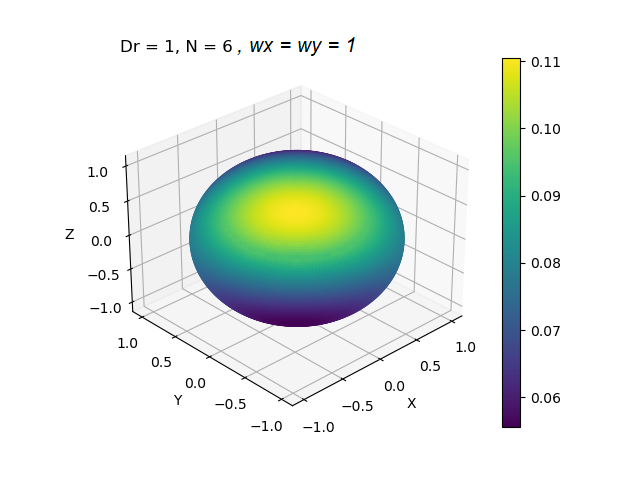
\includegraphics[scale=0.33]{Bilder_wxwy/Sol_onSphere_wx=1=wy_Dr=1_N=6}
	\end{minipage}
	\hfill 
	\begin{minipage}{0.4\textwidth}
		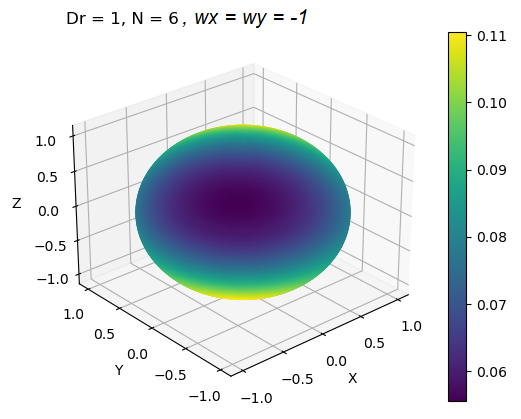
\includegraphics[scale=0.33]{Bilder_wxwy/Sol_onSphere_wx=-1=wy_Dr=1_N=6}
	\end{minipage}
    \end{figure}

	\begin{figure}[H]
	\centering
	\begin{minipage}{0.4\textwidth}
		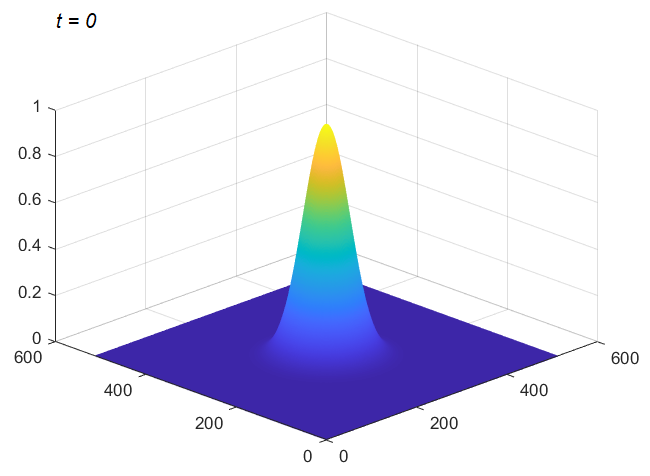
\includegraphics[scale=0.3]{Bilder_wxwy/t=0_wxwy=1_wxwy=-1}
	\end{minipage}
	\hfill 
	\begin{minipage}{0.4\textwidth}
		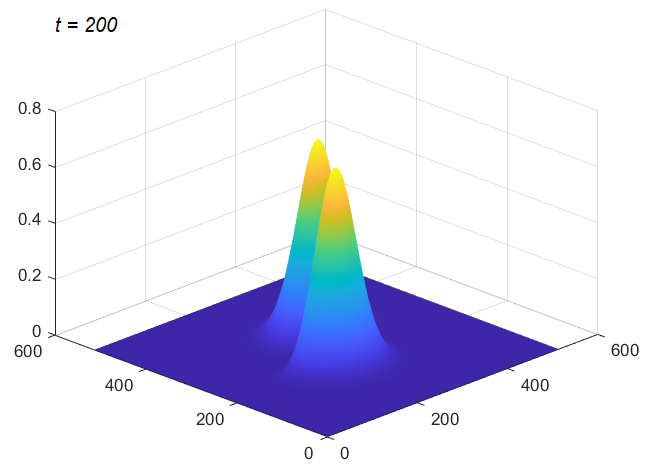
\includegraphics[scale=0.3]{Bilder_wxwy/t=200_wxwy=1_wxwy=-1}
	\end{minipage}
   \caption{Numerical results for $c^0_0$ at different times using $N=1$ and $D_r=1$. A cluster with higher particle density splits into two, each moving in opposite directions.}
    \end{figure}
\end{frame}

\begin{comment}
	\begin{frame}
		\scriptsize
		The matrix $\textcolor{red}{A}$ and the Matrix $\textcolor{red}{B}$ has the form \\
		\vspace{8pt}
		
		\[
		\begin{minipage}{0.45\linewidth}
			\[
			A = \begin{pmatrix}
				\vspace{8pt}
				0 & 0 & \frac{\sqrt{15}}{15} & 0 & 0 & 0 \\
				\vspace{8pt}
				0 & 0 & \frac{1}{7} & 0 & 0 & 0 \\
				\vspace{8pt}
				\frac{\sqrt{15}}{15} & \frac{1}{7} & 0 & \frac{\sqrt{3}}{21} & 0 &  0 \\
				\vspace{8pt}
				0 & 0 & \frac{\sqrt{3}}{21} & 0 & 0 & 0 \\
				\vspace{8pt}
				0 & 0 & 0 & 0 & 0 & \frac{1}{7} \\
				\vspace{8pt}
				0 & 0 & 0 & 0 & \frac{1}{7} & 0
			\end{pmatrix},
			\]
		\end{minipage}
		\begin{minipage}{0.45\linewidth}
			\[
			B = \begin{pmatrix}
				\vspace{8pt}
				0 & 0 & 0 & 0 & \frac{\sqrt{15}}{15} & 0 \\
				\vspace{8pt}
				0 & 0 & 0 & 0 & -\frac{1}{7} & 0 \\
				\vspace{8pt}
				0 & 0 & 0 & 0 & 0 &  \frac{1}{7} \\
				\vspace{8pt}
				0 & 0 & 0 & 0 & \frac{\sqrt{3}}{21} & 0 \\
				\vspace{8pt}
				\frac{\sqrt{15}}{15} & -\frac{1}{7} & 0 & \frac{\sqrt{3}}{21} & 0 & 0 \\
				\vspace{8pt}
				0 & 0 & \frac{1}{7} & 0 & 0 & 0
			\end{pmatrix}
			\]
		\end{minipage}
		\]
	\end{frame}
\end{comment}